%%%%%%%%%%%%%%%%%%%%%%%%%%%%%%%%%%%%%%%%%
% Simple Sectioned Essay Template
% LaTeX Template
%
% This template has been downloaded from:
% http://www.latextemplates.com
%
% Note:
% The \lipsum[#] commands throughout this template generate dummy text
% to fill the template out. These commands should all be removed when 
% writing essay content.
%
%%%%%%%%%%%%%%%%%%%%%%%%%%%%%%%%%%%%%%%%%

%----------------------------------------------------------------------------------------
%	PACKAGES AND OTHER DOCUMENT CONFIGURATIONS
%----------------------------------------------------------------------------------------

\documentclass[12pt]{article} % Default font size is 12pt, it can be changed here

\usepackage{geometry} % Required to change the page size to A4
\geometry{a4paper} % Set the page size to be A4 as opposed to the default US Letter

\usepackage{graphicx} % Required for including pictures

\usepackage{float} % Allows putting an [H] in \begin{figure} to specify the exact location of the figure
\usepackage{subcaption}
\usepackage{mwe}
\usepackage{wrapfig} % Allows in-line images such as the example fish picture

\usepackage{lipsum} % Used for inserting dummy 'Lorem ipsum' text into the template
%\usepackage{biblatex}
%\usepackage[backend=bibtex]{biblatex}

\linespread{1.2} % Line spacing

%\setlength\parindent{0pt} % Uncomment to remove all indentation from paragraphs

\graphicspath{{pictures/}} % Specifies the directory where pictures are stored


\begin{document}

\section {GeoCorrection Investigation}
	Images captured from satellites are extremely useful for a variety of reason. Many of these reasons include knowing the geographical location of the image. Due to the technical specifications of the cameras, we cannot know the precise latitude and longitude of the image. The precision is lost due to resolution, distortion, and other similar effects. There are techniques that have been tested to try and improve upon the precision of the latitude and longitude.

	The following text describes some techniques that can be used to correct the latitude and longitude of a given image. First I will describe the baseline routine, SIFT/SURF + RANSAC. I will then talk about two other techniques that try to improve the correction above this baseline.

\section{Baseline Algorithm}

\subsection{SIFT/SURF}
	When comparing images, a computer needs points of reference in both images. A widely used technique called Scale-Invariant Feature Transform (SIFT) was developed to create these points of reference. The SIFT technique uses Gaussian Blurring  to smooth the image on different scales, then takes the difference between those smoothed images. These differences help locate maximums and minimums in the image.
	%relies on finding maxima and minima of the difference in Gaussian blurring functions on different scales. 
	These extrema, called keypoints, are cataloged for the given image. An example of these keypoints is given in figure \ref{fig:Keypoints}.

\begin{figure}[h]
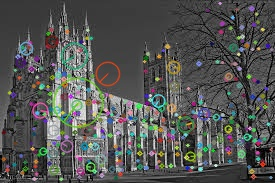
\includegraphics[width=\textwidth]{sift_keypoints.jpeg} 
\caption{An example of keypoints from the SIFT algorithm. Each circle is a keypoint, with the line from middle to edge designating a direction used for rotational matching}
\label{fig:Keypoints}
\end{figure}

	The SIFT algorithm is reliable, but it can be slow. SURF (Speeded-Up Robust Features) is a speed improvement on SIFT. It makes some approximations on the math to speed up the calculation of the keypoints, but it looses some of the precision of SIFT. Many programs that can do SIFT can also do SURF, so further testing to see if SURF is viable is needed.
		
	It is possible to see how well the keypoints match up between images. An example of this can be seen in figure \ref{fig:SIFT_match}. 
	
\begin{figure}[h]
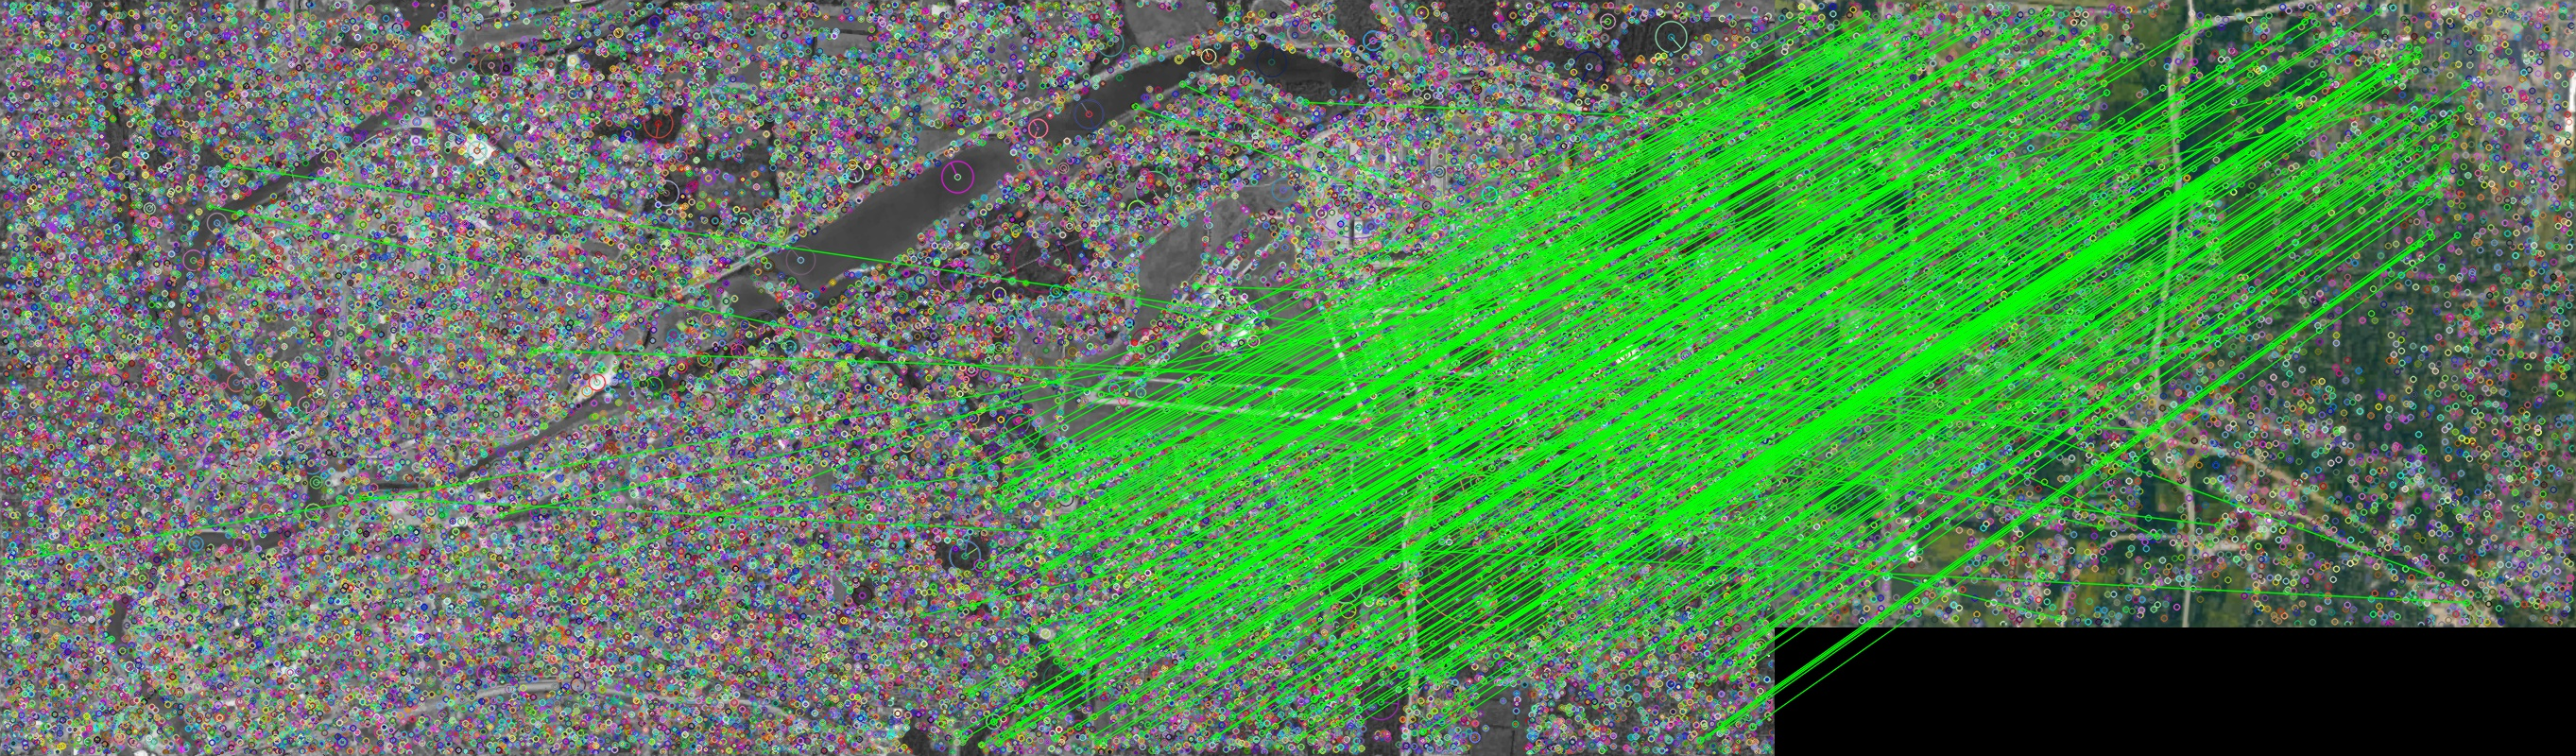
\includegraphics[width=\textwidth]{SIFT_matches.jpeg}
\caption{Keypoint matching. These two images have some overlap. The SIFT algorithm finds that overlap and draws green lines between the parts that overlap for visibility. }
\label{fig:SIFT_match}
\end{figure}

\subsection{Applying Corrections}
	After finding the keypoints from SIFT/SURF, there needs to be a way to test those keypoints against a keypoint template to correct the original image. The tested method for this is called RAndom SAmple Consensus (RANSAC). 
	
	RANSAC is an iterative algorithm that estimates parameters from a data set that contains outliers. RANSAC gives no weight to these outliers, allowing it to find a best fit on the real data points. For our method, RANSAC chooses N random pair points between the two images. After matching those points, the algorithm calculates how many other points are inliers (non-chosen keypoints match). A match is defined as two keypoints being within a set distance from each other. The algorithm does this random choosing of pair points until it has a maximum number of matching points for the two images. This mapping of keypoints gives a base transform to work with.
	
	After achieving a base transform, the original image may need to be transformed more to align better with the template. This means we need to calculate a homography between the two images. An algorithm calculates this homography between the two images, using a least-squares method. The least-squares method attempts to align all the keypoints by applying transformations to the image until we achieve the best match.

\subsection{Implementation}
	The current implementation of this process was done in OpenCV, which contains modules for both C++ and Python libraries. It contains both the SIFT and SURF algorithms to detect keypoints, as well as a matching algorithm to calculate the homography between two pictures. Implicit in the second algorithm is the RANSAC algorithm. 

	An an attempt to learn this software, I created an algorithm to make a panorama of the city of Dayton with images pulled from Google Earth, Figure \ref{fig:Panorama_individual}. The algorithm I created can read in images, calculate the keypoints, use the matching algorithm to create the homography between the images and stitch the images together. The final image can be seen in figure \ref{fig:panorama_total}
	
\begin{figure*}
\begin{subfigure}[t]{.5\textwidth}
\centering
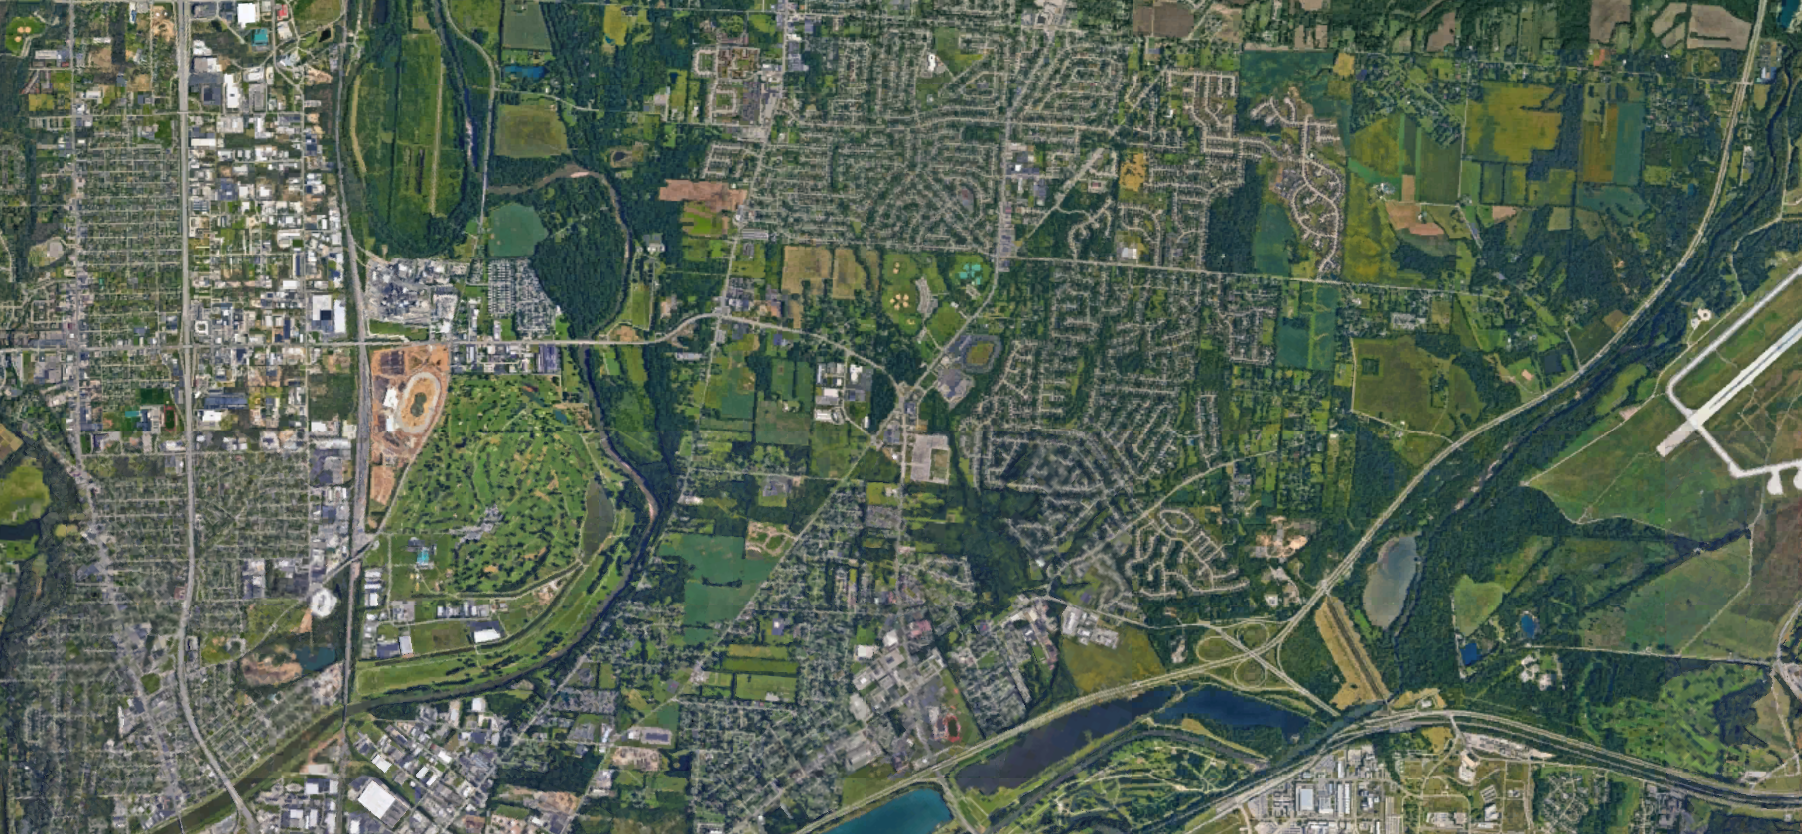
\includegraphics[width=\textwidth]{/Dayton_panorama/Map1.png}
\caption{First Image}
\end{subfigure}
\hfill
\begin{subfigure}[t]{.5\textwidth}
\centering
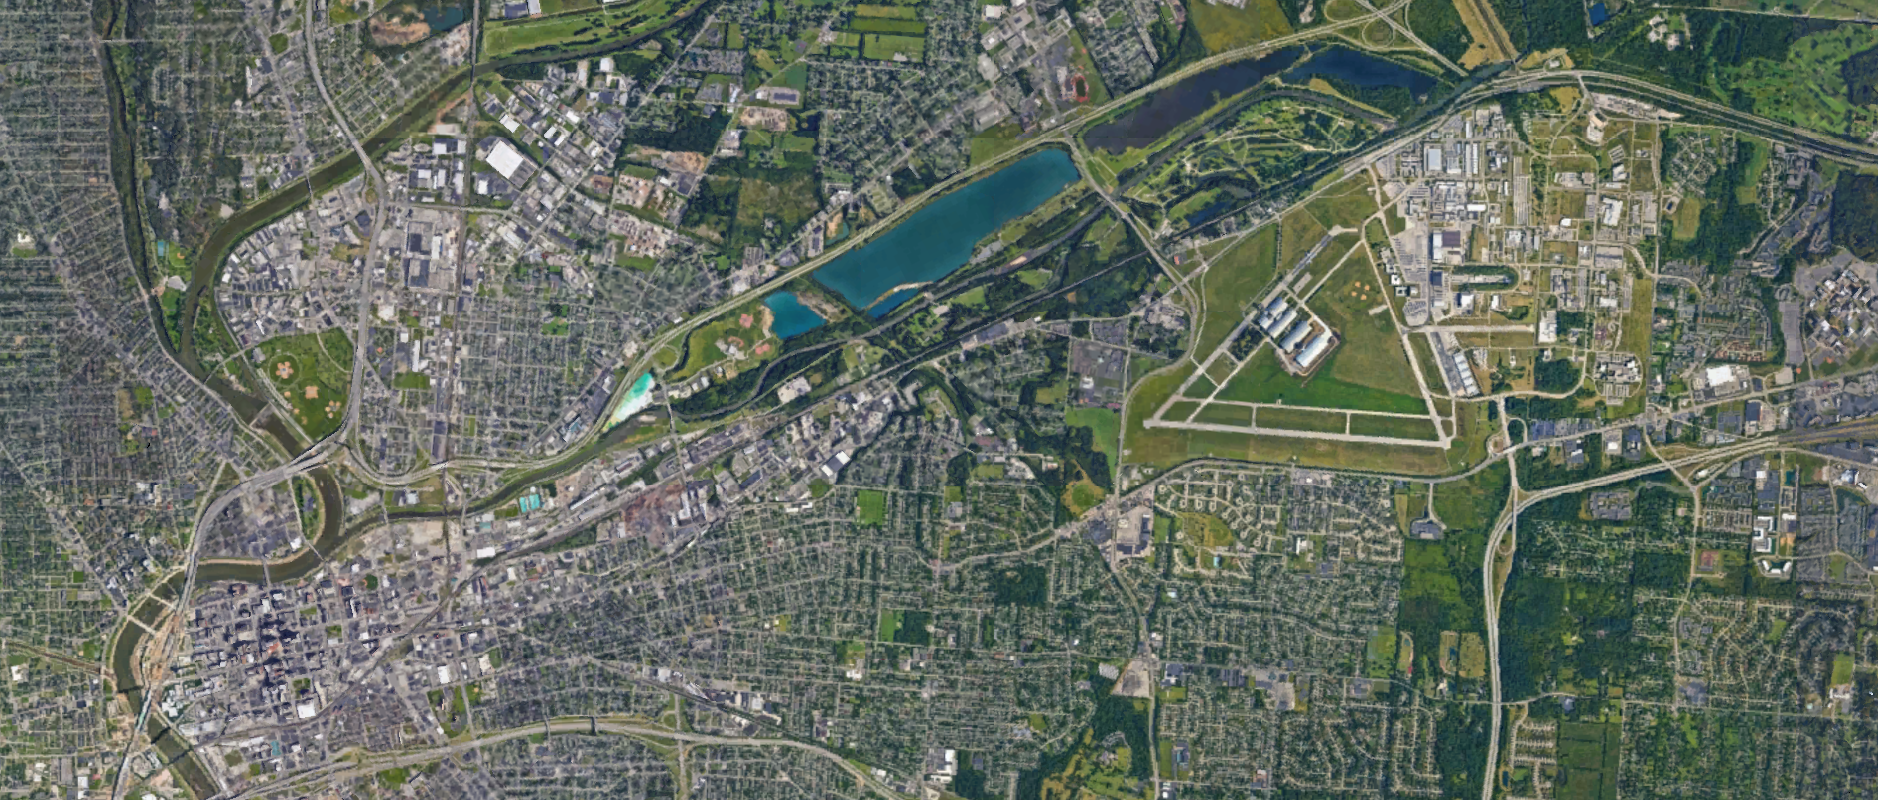
\includegraphics[width=\textwidth]{/Dayton_panorama/Map2.png}
\caption{Second Image}
\end{subfigure}

\begin{subfigure}[t]{.6\textwidth}
\centering
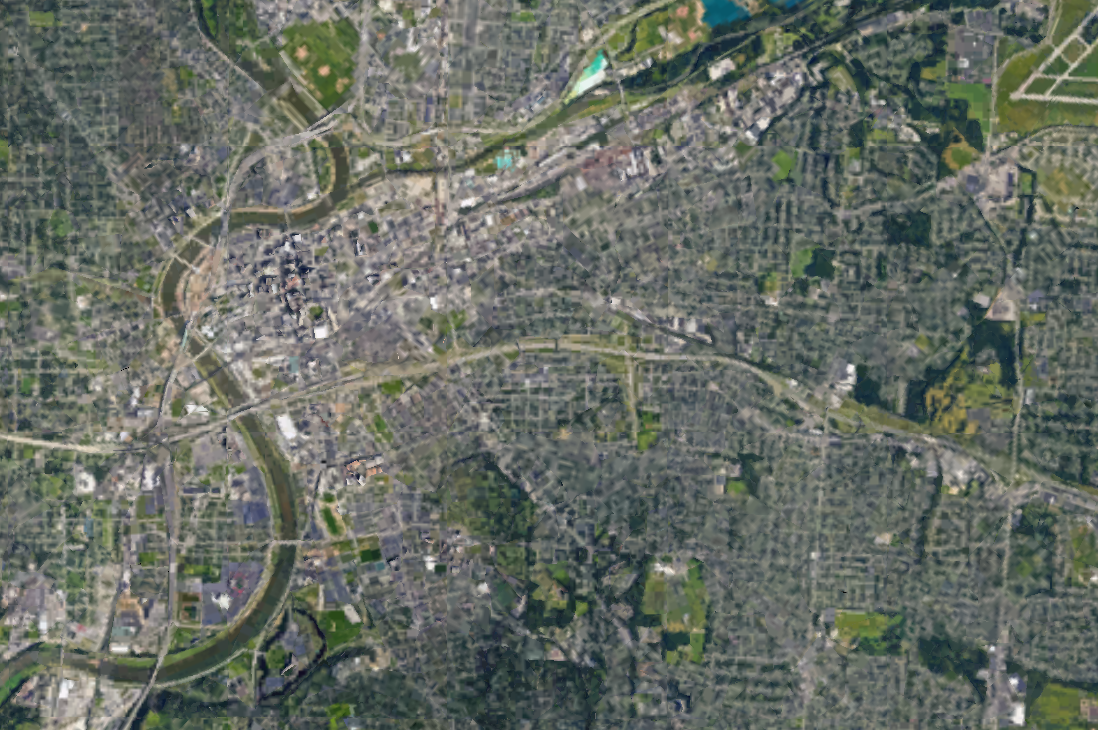
\includegraphics[width=\textwidth]{/Dayton_panorama/Map4.png}
\caption{Third Image}
\end{subfigure}


\caption{These images were taken from Google Earth. They have some overlap between all three images.}

\label{fig:Panorama_individual}
\end{figure*}

\begin{figure}[!h]
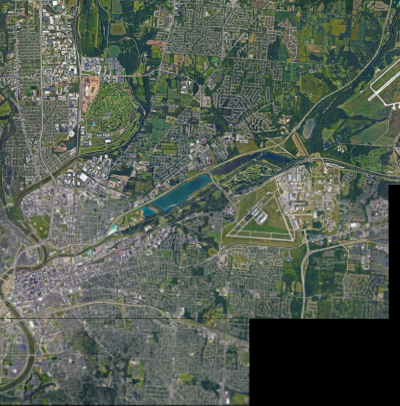
\includegraphics[width=\textwidth]{Dayton_panorama/total_stitch.png}
\caption{Images from figure \ref{fig:Panorama_individual} ran through the algorithm and transformed to form panoramic image}
\label{fig:panorama_total}
\end{figure}

As seen in figure \ref{fig:panorma_total}, the stitching program works well. It calculated where the overlay between all three images should be, shifted the images correctly and placed them on correctly on a canvas. This example was a simple x,y shift. This algorithm can also deal with distortions in the images as well. 

\section{Other Methods}
The previous method can be slow due to the number of templates/keypoints that need to be read in and analyzed before the correction occurs. There are various papers that also attempt to correct images using other methods. 

\subsection{Template Matching via GPU}
	Template matching is the 'brute force' way of finding similarities between two images. You have an image you wish to scan, and a smaller template to match to. You can 'slide' the template around pixel by pixel and calculate the goodness of fit for that overlay until you find the best fit. This concept is the easiest to understand, but can be very slow depending on the size of the image and the template. 
	
	A paper \cite{rs5094488} has found a way to speed up this process and push many of the calculations to the GPU. This technique involves convolving the source image with the template by using a Fast-Fourier Transform (FFT). This is done to speed up the process since convolving in the spatial domain is time-consuming but in the frequency domain it can be done by multiplication. A second FFT transforms the information back to the spatial domain. The convolution has a maximum at the center point where the template matches the source image. 
	
	This technique relies upon having ground information from sources such as GDAL to allow for the correction. The offsets are stored in GDAL's virtual file (VRT) and used to create the offset transformation to correct the location of the source image. '
		
	Whether this is faster than the baseline algorithm will require further testing. OpenCV has a template matching algorithm, but it may not work with the process described here.

\subsection{Color Invariant Transform}
	This technique is very similar to the baseline technique, but adds a new degree to the matches between images \cite{Setkov:2013:CIF:2466715.2466731}. This technique attempts to correct any color difference between images that may occur, such as different cameras. It adds a step to the baseline technique where it transforms the colors of the images before feature mapping. This claims to improve matching when the color scheme has been changed. This technique may not be as useful if different devices produce approximately the same color images.
	
\begin{figure}
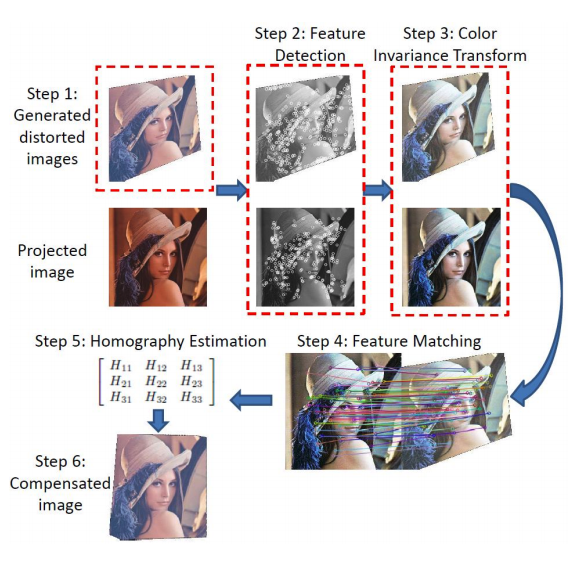
\includegraphics[width=\textwidth]{Color_invariant.png}
\caption{Taken from \cite{Setkov:2013:CIF:2466715.2466731}. It shows the steps taken by this algorithm to create an invariant color transform to help with feature matching.}
\label{fig:Color_invariant}
\end{figure}

\bibliographystyle{plain}
\bibliography{GeoCorrection}


\end{document}